\subsection{End to End Device Test}

One verification that all components of the proposed device work together was performed. A cylindrical rod was placed between the assembled devices
graspers at approximately 5cm distance from the camera and the detection program activated. If the device logged that the rod was detected 
at the expected position, and the graspers then closed, the test passed.

One mechanical alteration had to be made to the device for this test to be performed. As mentioned in Section \ref{sec:methods:collection-single},
small distances, less than a 2 to 3 hundred mm, cannot be detected by the device as originally designed due to the large stereo camera baseline.
For this test a new camera mount with a narrower baseline was fabricated and new calibration data for this mount was collected following
the procedure in Section \ref{sec:methods:calibration}. Changing the baseline changes the resolution of the stereo cameras depth measurement,
and the rate at which resolution changes vs distance, but it does not change the mechanism of detecting perches once a calibrated point cloud is 
produces. Therefore, the results in Sections \ref{sec:results:perch-rate} and \ref{sec:results:perch-accuracy} are still valid. 

One other change to the settings of the Hough transform was made for this test, to increase the resolution of its voting space.
Early testing revealed that the device failed to detect objects that were close enough to the cameras to be within range of the grasper, 
even with a smaller baseline and updated settings such that valid point cloud data was available for that near region. Fig. \ref{fig:e2e-bad}
shows sample data of such a test case. 

\begin{figure}[H]
    \centering
    % Generated from "C:\Users\wyatt\Documents\GVSU\Thesis\prototype testing\test bin files\test_7"
    \begin{subfigure}[b]{\textwidth}        
        \begin{subfigure}[b]{0.32\textwidth}
            \centering
            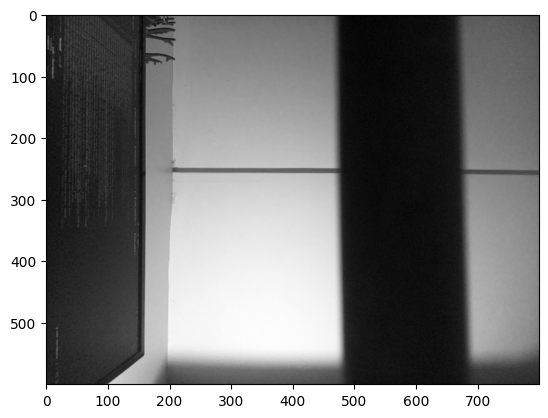
\includegraphics[width=\textwidth]{sections/methods/e2e-left-bad.png}
            \caption{Left camera image with zigzag background.}
            \label{fig:e2e-bad:img}
        \end{subfigure}
        \hfill
        \begin{subfigure}[b]{0.32\textwidth}
            \centering
            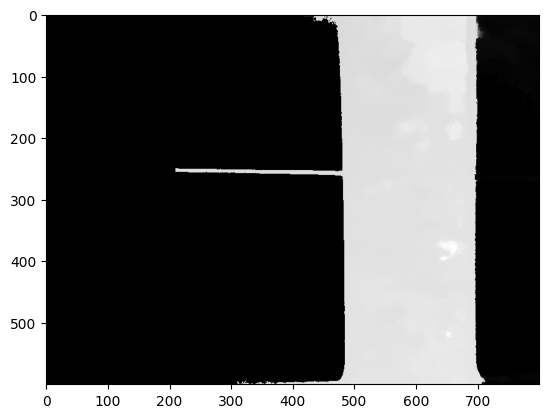
\includegraphics[width=\textwidth]{sections/methods/e2e-disp-bad.png}
            \caption{Disparity map calculated from \ref{fig:e2e-bad:img} and the corresponding right image.}
            \label{fig:e2e-bad:disp}
        \end{subfigure}
        \hfill
        \begin{subfigure}[b]{0.32\textwidth}
            \centering
            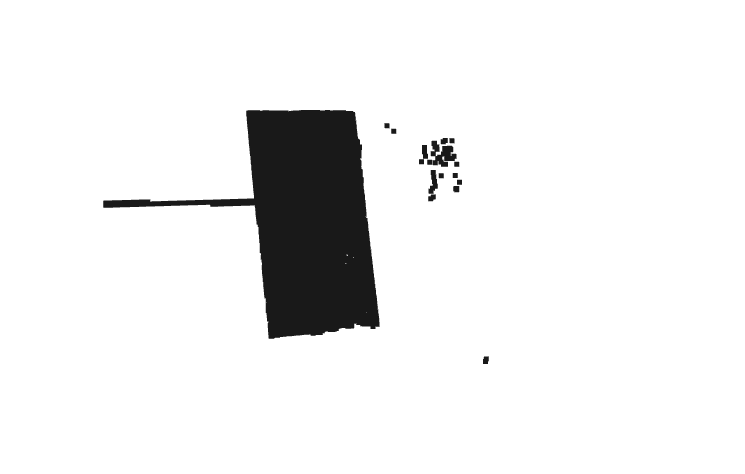
\includegraphics[width=\textwidth]{sections/methods/e2e-ptcld-bad.png}
            \caption{Point cloud produced from the disparity data in \ref{fig:e2e-bad:disp}.}
            \label{fig:e2e-bad:ptcld}
        \end{subfigure}
    \end{subfigure}
    \caption{Sample data showing failure to detect a perch at close range. \ref{fig:e2e-bad:img} shows the grayscale image from the left
    camera, with a perch roughly 5cm away. \ref{fig:e2e-bad:disp} shows the disparity data in which the object was clearly detected with 
    high disparity, however the point cloud in \ref{fig:e2e-bad:ptcld} shows that it was not detected by the Hough transform as a candidate
    (it is not shaded any color and no blue line is drawn through it).}
    \label{fig:e2e-bad}
\end{figure}

It was noticed that the Cartesian voting space resolution was roughly 5.7 cm with the default granularity setting of 128 subdivisions
(default settings used are shown in table \ref{tab:hough-args}), which is roughly the same size as the range of distances where
the grasper can close around a perch. To see if the resolution of the Hough space was causing this failure, the parameters 
were changes so that the voting space resolution was 10mm. After this change the perch was successfully detected. Images of the 
successful detection are shown in Fig. \ref{fig:e2e-good}. 


\begin{figure}[H]
    \centering
    % Generated from "C:\Users\wyatt\Documents\GVSU\Thesis\prototype testing\test bin files\test_7"
    \begin{subfigure}[b]{\textwidth}        
        \begin{subfigure}[b]{0.32\textwidth}
            \centering
            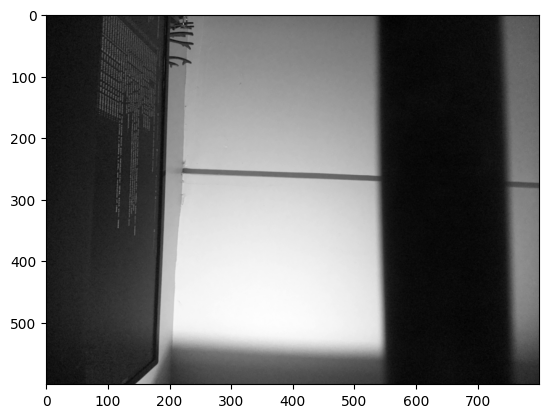
\includegraphics[width=\textwidth]{sections/methods/e2e-left-good.png}
            \caption{Left camera image with zigzag background.}
            \label{fig:e2e-good:img}
        \end{subfigure}
        \hfill
        \begin{subfigure}[b]{0.32\textwidth}
            \centering
            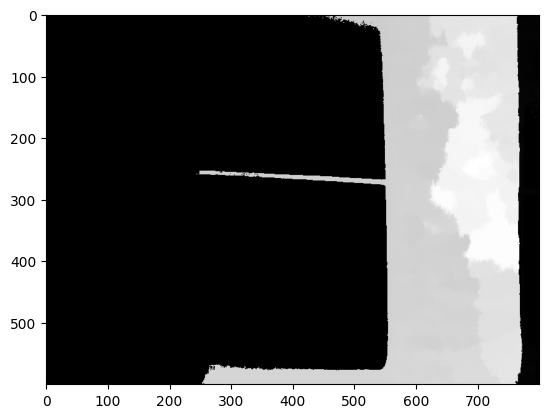
\includegraphics[width=\textwidth]{sections/methods/e2e-disp-good.png}
            \caption{Disparity map calculated from \ref{fig:e2e-good:img} and the corresponding right image.}
            \label{fig:e2e-good:disp}
        \end{subfigure}
        \hfill
        \begin{subfigure}[b]{0.32\textwidth}
            \centering
            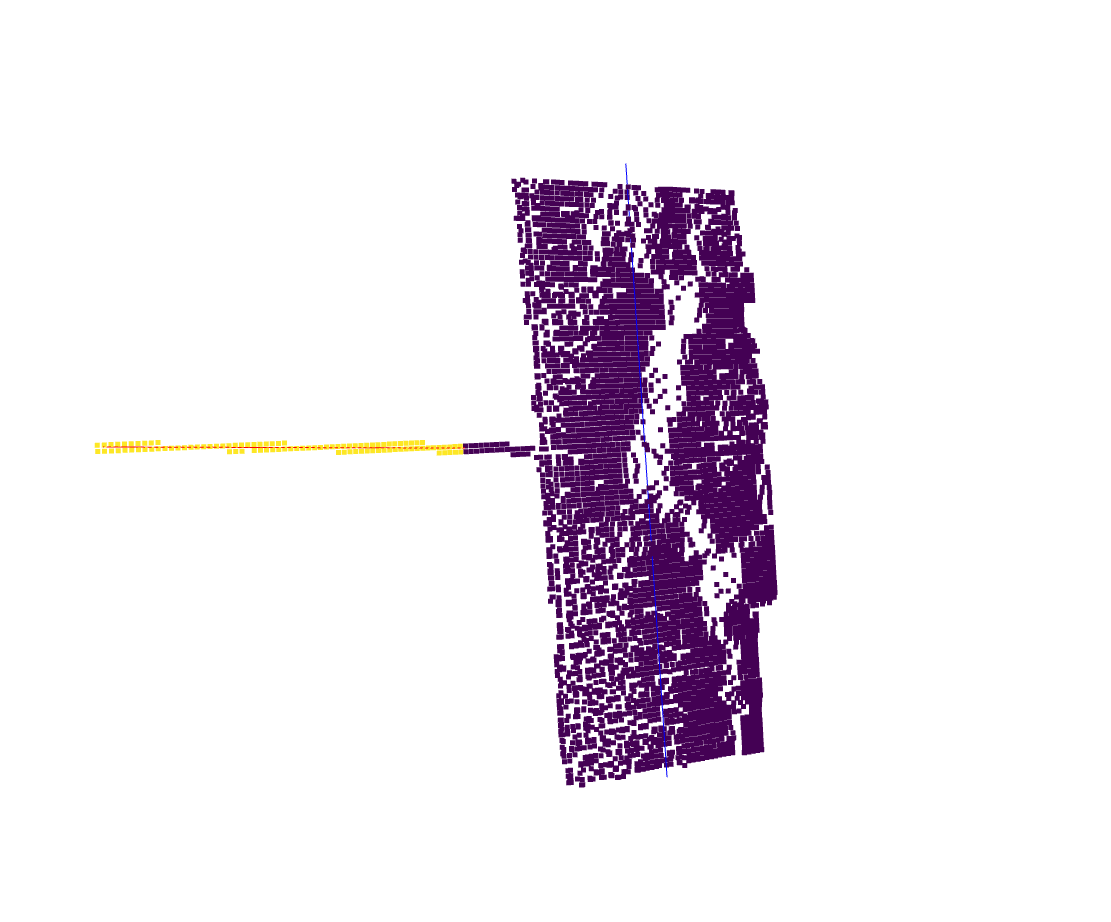
\includegraphics[width=\textwidth]{sections/methods/e2e-ptcld-good.png}
            \caption{Point cloud produced from the disparity data in \ref{fig:e2e-good:disp}.}
            \label{fig:e2e-good:ptcld}
        \end{subfigure}
    \end{subfigure}
    \caption{Sample data showing a successful perch detection at close range after increasing the Hough space resolution. \ref{fig:e2e-good:img} shows the left camera image
    of a perch roughly 5cm away, similar to Fig. \ref{fig:e2e-bad:img}. Like in Fig. \ref{fig:e2e-bad:disp}, \ref{fig:e2e-good:disp}
    shows the object clearly detected. After the resolution increase, the perch is now successfuly detected and marked in \ref{fig:e2e-good:ptcld}.}
    \label{fig:e2e-good}
\end{figure}